\documentclass[single]{ubook}
\usepackage{lipsum}
\usepackage{svg}
\begin{document}
\thispagestyle{plain}
\utitle{Title of Example Note}
\section{Chapter 1}\label{a:temp1}
\lettrine[lines=2, nindent=0pt, findent=0.5em]{S}{ee} \lipsum[1]\marginpar{Nam dui ligula, fringilla a, euismod sodales, sollicitudin vel, wisi. Morbiauctor lorem non justo. Nam lacus libero, pretium at, lobortis vitae, ultri
cies et, tellus.}
\begin{align}
  \mathcal{N}(\mu, \sigma) = \frac{1}{\sqrt{2\pi}\sigma}\exp\biggl[\frac{(x-\mu)^2}{\sigma^2}\biggr]
  % \sum_{n=1}^{100} \prod_{i=1}^{100} n \times i
\end{align}
\lipsum[1]\footnote[1]{Lorem ipsum dolor sit amet, consectetuer adipiscing elit. Ut purus elit, vestibulum ut, place-
rat ac, adipiscing vitae, feli.}

\begin{theorem}{Test}
  True is false, false is true.
\end{theorem}
\lipsum[1]
\begin{enumerate}
  \item Lorem ipsum dolor sit amet, consectetuer adipiscing elit
  \item Praesent eget sem vel leo ultrices bibendum. Aenean faucibus. Morbi dolor nulla,
  malesuada eu, pulvinar at, mollis ac, nulla
  \item Ut purus elit, vestibulum ut, placerat ac, adipiscing vitae, felis
\end{enumerate}
\lipsum[1]
\begin{figure}[h]
  \centering
  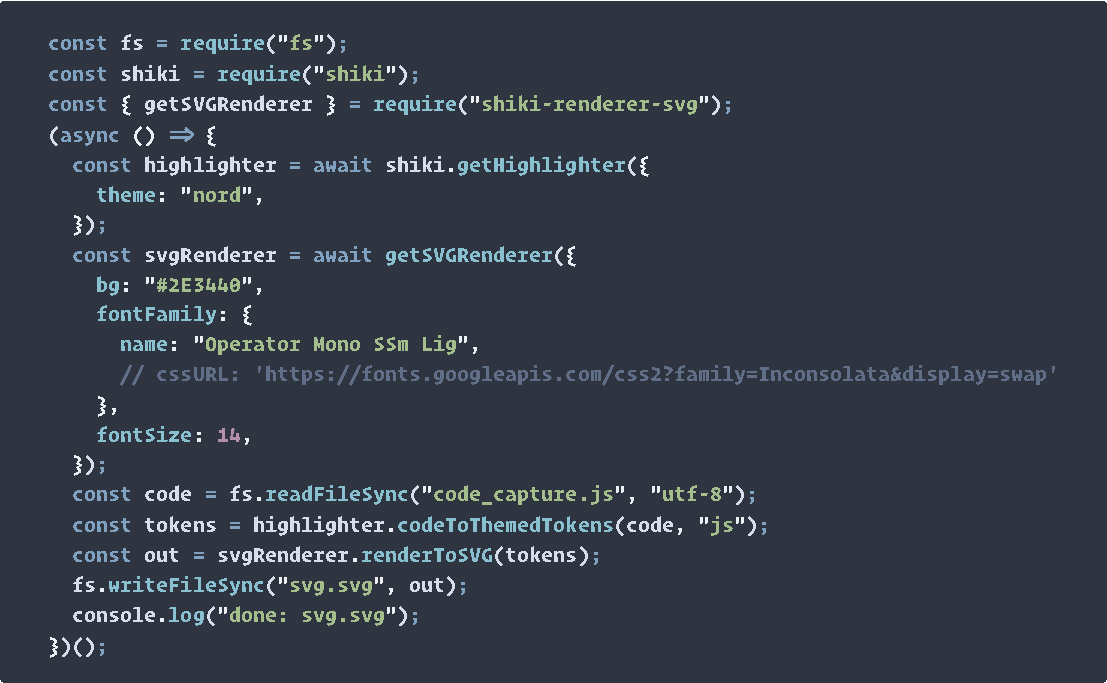
\includegraphics[width=\linewidth]{cc/svg.pdf}
  \caption{code for generating the svg file}
\end{figure}
\lipsum[1-5]\ref{a:temp1}
\url{https://google.com}
\end{document}